%%%%%%%%%%%%%%%%%%%%%%%%%%%%%%%%%%%%%%%%%%%%%%%%%%%%%%%%%%%%%%%%%%%%%%%%%%%%%%%
% ARCHITECTURE DIAGRAMS - COMPLETE SIMULATION DESIGN
% 仿真架构图集 - Inbound, Outbound, 总体设计
%%%%%%%%%%%%%%%%%%%%%%%%%%%%%%%%%%%%%%%%%%%%%%%%%%%%%%%%%%%%%%%%%%%%%%%%%%%%%%%
% 包含3个TikZ架构图:
% 1. Inbound流程架构 (Figure 4.X-A)
% 2. Outbound流程架构 (Figure 4.X-B)
% 3. 总体仿真设计架构 (Figure 4.X-C) - Entity, Process, Constraint
%%%%%%%%%%%%%%%%%%%%%%%%%%%%%%%%%%%%%%%%%%%%%%%%%%%%%%%%%%%%%%%%%%%%%%%%%%%%%%%
% REQUIRES: \usepackage{tikz}
%           \usetikzlibrary{shapes,arrows,positioning,fit,backgrounds}
%%%%%%%%%%%%%%%%%%%%%%%%%%%%%%%%%%%%%%%%%%%%%%%%%%%%%%%%%%%%%%%%%%%%%%%%%%%%%%%

%=============================================================================
% DIAGRAM 1: INBOUND PROCESS ARCHITECTURE
% Inbound流程: Truck Arrival → Timeslot Allocation → Unloading → FTE Processing
%=============================================================================

\begin{figure}[h]
    \centering
    \scalebox{0.85}{  % 缩小到85%以适应页面
    \begin{tikzpicture}[
        node distance=1.5cm,  % 减小节点间距
        entity/.style={rectangle, draw, fill=blue!15, text width=2.3cm, text centered, rounded corners, minimum height=0.9cm, thick},
        process/.style={rectangle, draw, fill=green!20, text width=2.6cm, text centered, minimum height=0.95cm, thick},
        resource/.style={ellipse, draw, fill=orange!20, text width=2cm, text centered, minimum height=0.8cm, thick},
        constraint/.style={rectangle, draw, fill=red!15, text width=2.2cm, text centered, minimum height=0.75cm, dashed, thick},
        arrow/.style={->, >=stealth, thick},
        darrow/.style={->, >=stealth, thick, dashed, red}
    ]
        % ========== Main Flow (Left to Right) ==========
        % Stage 1: Arrival
        \node[entity] (arrival) {Truck Arrival\\(Poisson $\lambda_h$)};
        
        % Stage 2: Queue for Timeslot
        \node[process, right=2cm of arrival] (queue) {Queue for\\Reception Timeslot};
        
        % Stage 3: Unloading at Dock
        \node[process, right=2cm of queue] (unload) {Unloading\\(30 min)};
        
        % Stage 4: FTE Processing
        \node[process, right=2cm of unload] (processing) {FTE Process\\(24h limit)};
        
        % Stage 5: Completion
        \node[entity, right=2cm of processing] (complete) {Complete};
        
        % ========== Resources (Top) ==========
        \node[resource, above=1.8cm of queue] (timeslot) {Reception\\Timeslot\\Capacity};
        
        \node[resource, above=1.8cm of processing] (fte) {FTE Inbound\\Capacity\\(hourly)};
        
        % ========== Constraints (Bottom) ==========
        \node[constraint, below=1.5cm of queue] (timeslot_const) {Hourly\\Timeslot Limit\\(FG: 2, R\&P: 1)};
        
        \node[constraint, below=1.5cm of processing] (deadline) {24-hour\\Processing\\Deadline};
        
        % ========== Main Flow Arrows ==========
        \draw[arrow] (arrival) -- (queue);
        \draw[arrow] (queue) -- node[above, font=\small] {Allocated} (unload);
        \draw[arrow] (unload) -- node[above, font=\small] {Unloaded} (processing);
        \draw[arrow] (processing) -- (complete);
        
        % ========== Resource Constraint Arrows ==========
        \draw[darrow] (timeslot) -- node[right, font=\footnotesize] {Constrains} (queue);
        \draw[darrow] (fte) -- node[right, font=\footnotesize] {Constrains} (processing);
        
        % ========== Constraint Links ==========
        \draw[darrow] (timeslot_const) -- (queue);
        \draw[darrow] (deadline) -- (processing);
        
    \end{tikzpicture}
    }  % 结束scalebox
    \caption{Inbound process architecture: truck arrival, timeslot allocation, unloading, and FTE-constrained processing with 24-hour deadline.}
    \label{fig:inbound_architecture}
\end{figure}

%=============================================================================
% DIAGRAM 2: OUTBOUND PROCESS ARCHITECTURE
% Outbound流程: Truck Arrival → FTE Processing → Timeslot Allocation → Loading → Departure
%=============================================================================

\begin{figure}[h]
    \centering
    \scalebox{0.82}{  % 缩小到82%以适应页面
    \begin{tikzpicture}[
        node distance=1.5cm,  % 减小节点间距
        entity/.style={rectangle, draw, fill=blue!15, text width=2.3cm, text centered, rounded corners, minimum height=0.9cm, thick},
        process/.style={rectangle, draw, fill=green!20, text width=2.6cm, text centered, minimum height=0.95cm, thick},
        resource/.style={ellipse, draw, fill=orange!20, text width=2cm, text centered, minimum height=0.8cm, thick},
        constraint/.style={rectangle, draw, fill=red!15, text width=2.2cm, text centered, minimum height=0.75cm, dashed, thick},
        decision/.style={diamond, draw, fill=purple!15, text width=1.6cm, text centered, minimum height=1.2cm, aspect=2, thick},
        arrow/.style={->, >=stealth, thick},
        darrow/.style={->, >=stealth, thick, dashed, red}
    ]
        % ========== Main Flow (Left to Right) ==========
        % Stage 1: Arrival
        \node[entity] (arrival) {Truck Arrival\\(Mixed: 75\% Scheduled\\+ 25\% Poisson)};
        
        % Stage 2: FTE Processing
        \node[process, right=2cm of arrival] (processing) {FTE Process\\(Prepare)};
        
        % Stage 3: Queue for Loading
        \node[process, right=2cm of processing] (queue) {Queue for\\Loading Slot};
        
        % Stage 4: Loading at Dock
        \node[process, right=2cm of queue] (loading) {Loading\\(30 min)};
        
        % Stage 5: Departure Check
        \node[decision, right=2cm of loading] (check) {SLA\\Check};
        
        % Stage 6: Departure
        \node[entity, right=1.8cm of check] (depart) {Departure};
        
        % ========== Resources (Top) ==========
        \node[resource, above=1.8cm of processing] (fte) {FTE Outbound\\Capacity\\(hourly)};
        
        \node[resource, above=1.8cm of queue] (timeslot) {Loading\\Timeslot\\Capacity};
        
        % ========== Constraints (Bottom) ==========
        \node[constraint, below=1.5cm of queue] (timeslot_const) {Hourly\\Timeslot Limit\\(FG: 1, R\&P: 4-6)};
        
        \node[constraint, below=1.5cm of check] (sla) {FG Departure\\Deadline\\(G2: same-day\\ROW: next-day)};
        
        % ========== Main Flow Arrows ==========
        \draw[arrow] (arrival) -- (processing);
        \draw[arrow] (processing) -- node[above, font=\small] {Ready} (queue);
        \draw[arrow] (queue) -- node[above, font=\small] {Allocated} (loading);
        \draw[arrow] (loading) -- (check);
        \draw[arrow] (check) -- (depart);
        
        % ========== SLA Miss Path ==========
        \node[entity, below=2.5cm of check, fill=red!20] (delayed) {Delayed\\(SLA Miss)};
        \draw[arrow, red] (check) -- node[right, font=\footnotesize] {Late} (delayed);
        \draw[arrow] (delayed) -| (depart);
        
        % ========== Resource Constraint Arrows ==========
        \draw[darrow] (fte) -- node[right, font=\footnotesize] {Constrains} (processing);
        \draw[darrow] (timeslot) -- node[right, font=\footnotesize] {Constrains} (queue);
        
        % ========== Constraint Links ==========
        \draw[darrow] (timeslot_const) -- (queue);
        \draw[darrow] (sla) -- (check);
        
    \end{tikzpicture}
    }  % 结束scalebox
    \caption{Outbound process architecture: truck arrival (mixed scheduled + random), FTE-constrained processing, timeslot allocation, loading, and SLA-based departure deadline check. G2 region requires same-day departure, ROW allows next-day.}
    \label{fig:outbound_architecture}
\end{figure}

%=============================================================================
% DIAGRAM 3: OVERALL SIMULATION DESIGN ARCHITECTURE
% 总体架构: Entity类型 → Process流程 → Constraint约束 → 并发管理
%=============================================================================

\begin{figure}[p]
    \centering
    \scalebox{0.75}{  % 缩小到75%以适应页面
    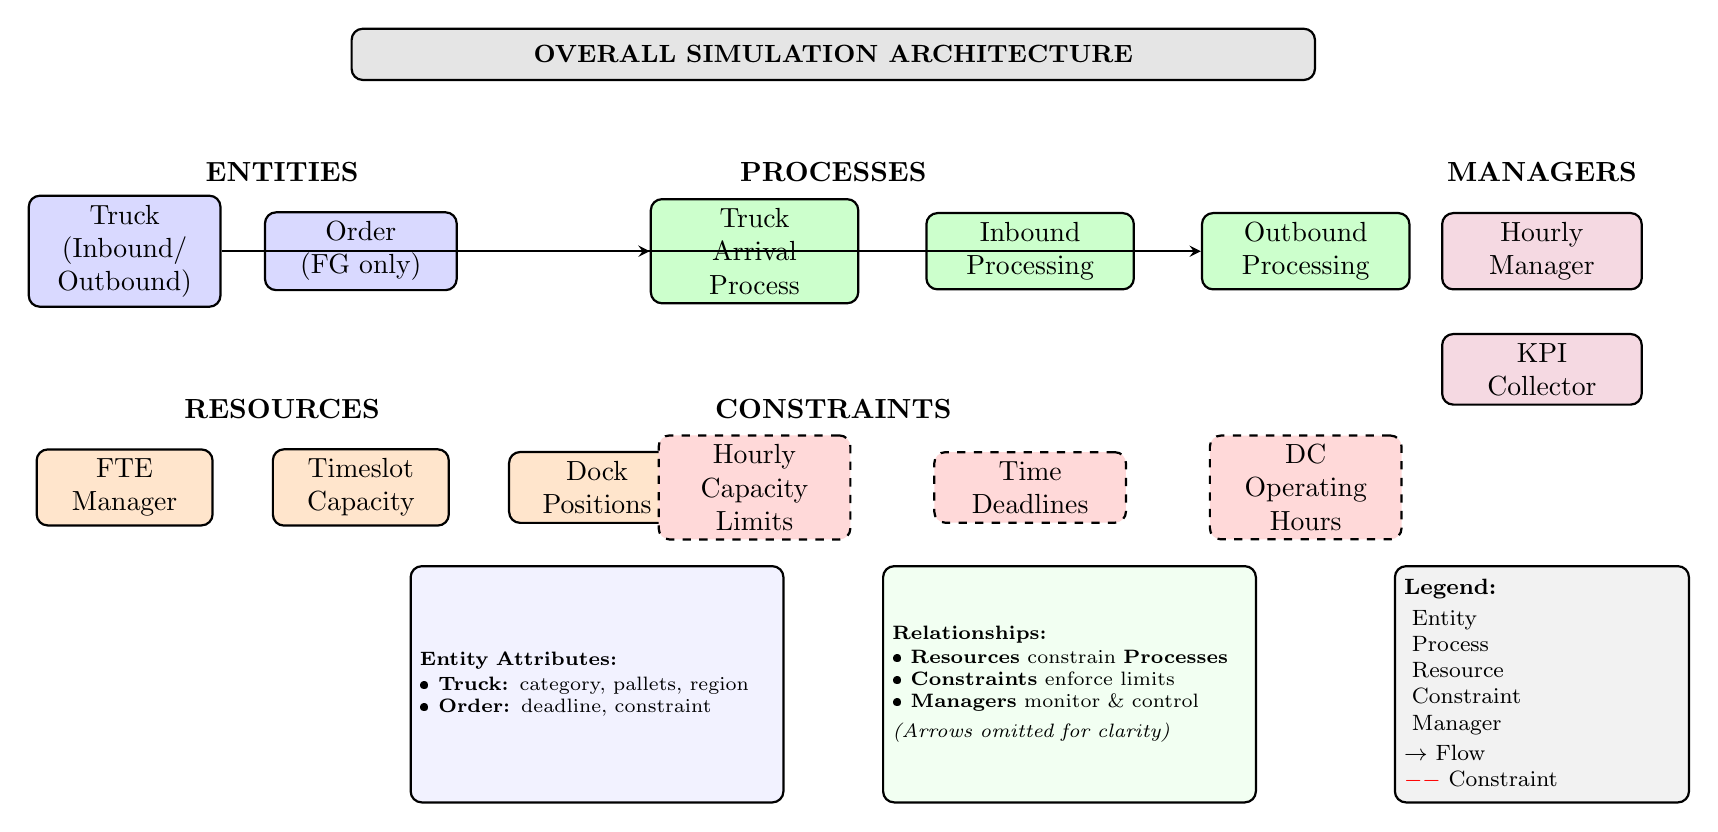
\begin{tikzpicture}[
        node distance=1.3cm,  % 减小节点间距
        box/.style={rectangle, draw, text width=2.2cm, text centered, rounded corners, minimum height=0.8cm, thick},
        entity/.style={box, fill=blue!15},
        process/.style={box, fill=green!20, text width=2.4cm},
        resource/.style={box, fill=orange!20, text width=2cm},
        constraint/.style={box, fill=red!15, dashed},
        manager/.style={box, fill=purple!15, text width=2.3cm},
        arrow/.style={->, >=stealth, thick},
        darrow/.style={->, >=stealth, thick, dashed}
    ]
        % ========== TITLE BOXES (Top Layer) ==========
        \node[box, fill=gray!20, text width=12cm, minimum height=0.65cm, font=\bfseries\small] at (0, 6.5) 
            {OVERALL SIMULATION ARCHITECTURE};
        
        % ========== LAYER 1: ENTITY TYPES (Top) ==========
        \node[font=\bfseries] at (-7, 5) {ENTITIES};
        
        \node[entity] at (-9, 4) (truck) {Truck\\(Inbound/\\Outbound)};
        \node[entity] at (-6, 4) (order) {Order\\(FG only)};
        
        % ========== LAYER 2: PROCESS TYPES (Middle-Top) ==========
        \node[font=\bfseries] at (0, 5) {PROCESSES};
        
        \node[process] at (-1, 4) (arrival) {Truck\\Arrival\\Process};
        \node[process] at (2.5, 4) (inbound_p) {Inbound\\Processing};
        \node[process] at (6, 4) (outbound_p) {Outbound\\Processing};
        
        % ========== LAYER 3: RESOURCE TYPES (Middle-Bottom) ==========
        \node[font=\bfseries] at (-7, 2) {RESOURCES};
        
        \node[resource] at (-9, 1) (fte_res) {FTE\\Manager};
        \node[resource] at (-6, 1) (timeslot_res) {Timeslot\\Capacity};
        \node[resource] at (-3, 1) (dock_res) {Dock\\Positions};
        
        % ========== LAYER 4: CONSTRAINT TYPES (Bottom) ==========
        \node[font=\bfseries] at (0, 2) {CONSTRAINTS};
        
        \node[constraint] at (-1, 1) (hourly_c) {Hourly\\Capacity\\Limits};
        \node[constraint] at (2.5, 1) (time_c) {Time\\Deadlines};
        \node[constraint] at (6, 1) (operating_c) {DC\\Operating\\Hours};
        
        % ========== LAYER 5: SIMULATION MANAGERS (Bottom) ==========
        \node[font=\bfseries] at (9, 5) {MANAGERS};
        
        \node[manager] at (9, 4) (hour_mgr) {Hourly\\Manager};
        \node[manager] at (9, 2.5) (kpi_mgr) {KPI\\Collector};
        
        % ========== CONNECTIONS: 仅保留核心流程箭头,避免遮挡 ==========
        % 只画 Entities → Processes 的直接流程
        \draw[arrow] (truck) -- (arrival);
        \draw[arrow] (order) -- (outbound_p);
        
        % NOTE: Resource/Constraint/Manager 的约束关系通过颜色编码和说明框表达
        % 不绘制交叉箭头,避免遮挡文字框
        
        % ========== LEGEND (Bottom Right) ==========
        \node[box, fill=gray!10, text width=3.5cm, minimum height=3cm, align=left, font=\footnotesize] at (9, -1.5) {
            \textbf{Legend:}\\[0.05cm]
            \textcolor{blue!70}{$\blacksquare$} Entity\\
            \textcolor{green!70}{$\blacksquare$} Process\\
            \textcolor{orange!70}{$\blacksquare$} Resource\\
            \textcolor{red!70}{$\blacksquare$} Constraint\\
            \textcolor{purple!70}{$\blacksquare$} Manager\\[0.05cm]
            $\rightarrow$ Flow\\
            \textcolor{red}{$- -$} Constraint
        };
        
        % ========== DETAILED BREAKDOWN BOXES (Bottom Left) ==========
        \node[box, fill=blue!5, text width=4.5cm, minimum height=3cm, align=left, font=\scriptsize] at (-3, -1.5) {
            \textbf{Entity Attributes:}\\[0.03cm]
            • \textbf{Truck:} category, pallets, region\\
            • \textbf{Order:} deadline, constraint
        };
        
        \node[box, fill=green!5, text width=4.5cm, minimum height=3cm, align=left, font=\scriptsize] at (3, -1.5) {
            \textbf{Relationships:}\\[0.03cm]
            • \textbf{Resources} constrain \textbf{Processes}\\
            • \textbf{Constraints} enforce limits\\
            • \textbf{Managers} monitor \& control\\[0.1cm]
            \textit{(Arrows omitted for clarity)}
        };
        
    \end{tikzpicture}
    }  % 结束scalebox
    \caption{Overall simulation design architecture showing entity types (Truck, Order), process flows (Arrival, Inbound, Outbound), resource managers (FTE, Timeslot, Dock), constraint mechanisms (Hourly capacity, Time deadlines, Operating hours), and concurrent management processes (Hourly manager, KPI collector). Solid arrows represent entity/data flow, dashed red arrows indicate constraint enforcement, dotted blue arrows show monitoring/control.}
    \label{fig:simulation_architecture_overview}
\end{figure}

%%%%%%%%%%%%%%%%%%%%%%%%%%%%%%%%%%%%%%%%%%%%%%%%%%%%%%%%%%%%%%%%%%%%%%%%%%%%%%%
% USAGE NOTES
%%%%%%%%%%%%%%%%%%%%%%%%%%%%%%%%%%%%%%%%%%%%%%%%%%%%%%%%%%%%%%%%%%%%%%%%%%%%%%%
% 
% 插入位置建议:
% ─────────────────────────────────────────────────────────────────────────────
% 1. Figure 4.X-A (Inbound Architecture)
%    位置: Section 4.3.X - Inbound Process Model
%    目的: 详细说明Inbound流程的各个阶段和约束
%
% 2. Figure 4.X-B (Outbound Architecture)  
%    位置: Section 4.3.X - Outbound Process Model
%    目的: 详细说明Outbound流程的各个阶段和SLA检查
%
% 3. Figure 4.X-C (Overall Architecture)
%    位置: Section 4.3 - Model Architecture (总览章节)
%    目的: 高层次展示整个仿真模型的组成要素和交互关系
%
% 推荐顺序:
% ─────────────────────────────────────────────────────────────────────────────
% 第一步: 插入总体架构图 (Figure 4.X-C) 在4.3节开头
%   - 给读者整体概念
%   - 展示Entity, Process, Resource, Constraint四大类组件
%
% 第二步: 插入Inbound和Outbound架构图 (Figures 4.X-A, 4.X-B) 在各自章节
%   - 深入讲解具体流程
%   - 补充技术细节
%
% 三图对比:
% ─────────────────────────────────────────────────────────────────────────────
% │ 图名              │ 层次   │ 关注点                    │ 适合章节    │
% ├──────────────────┼────────┼───────────────────────────┼─────────────┤
% │ Inbound Arch     │ 详细   │ 时间序列流程, 24h deadline│ 4.3.X       │
% │ Outbound Arch    │ 详细   │ 两阶段流程, SLA检查        │ 4.3.X       │
% │ Overall Arch     │ 总览   │ 组件类型, 交互关系         │ 4.3 总览    │
%
% 关键差异:
% ─────────────────────────────────────────────────────────────────────────────
% Inbound特点:
%   - 24小时处理deadline
%   - 单一流程:Arrival → Timeslot → Unload → Process
%
% Outbound特点:
%   - 两阶段流程:先Process后Loading(与Inbound相反)
%   - SLA检查(FG按region分类:G2 same-day, ROW next-day)
%   - 混合到达模式(75% scheduled + 25% random)
%
% Overall特点:
%   - 抽象层次:展示Entity/Process/Resource/Constraint分类
%   - 全局视角:包含所有管理器(Hourly, KPI)
%   - 交互关系:实线=流程,虚线=约束,点线=监控
%
%%%%%%%%%%%%%%%%%%%%%%%%%%%%%%%%%%%%%%%%%%%%%%%%%%%%%%%%%%%%%%%%%%%%%%%%%%%%%%%
% END OF ARCHITECTURE DIAGRAMS
%%%%%%%%%%%%%%%%%%%%%%%%%%%%%%%%%%%%%%%%%%%%%%%%%%%%%%%%%%%%%%%%%%%%%%%%%%%%%%%
